\section{Auswertung}
\label{sec:Auswertung}
\subsection{Fourier-Synthese}
Mit den berechneten Verhältnissen ergeben sich beim Einstellen der Rechteckspannung die in Abbildung \ref{fig:recht} dargestellte Funktion.

\begin{figure}[H]
  \centering
  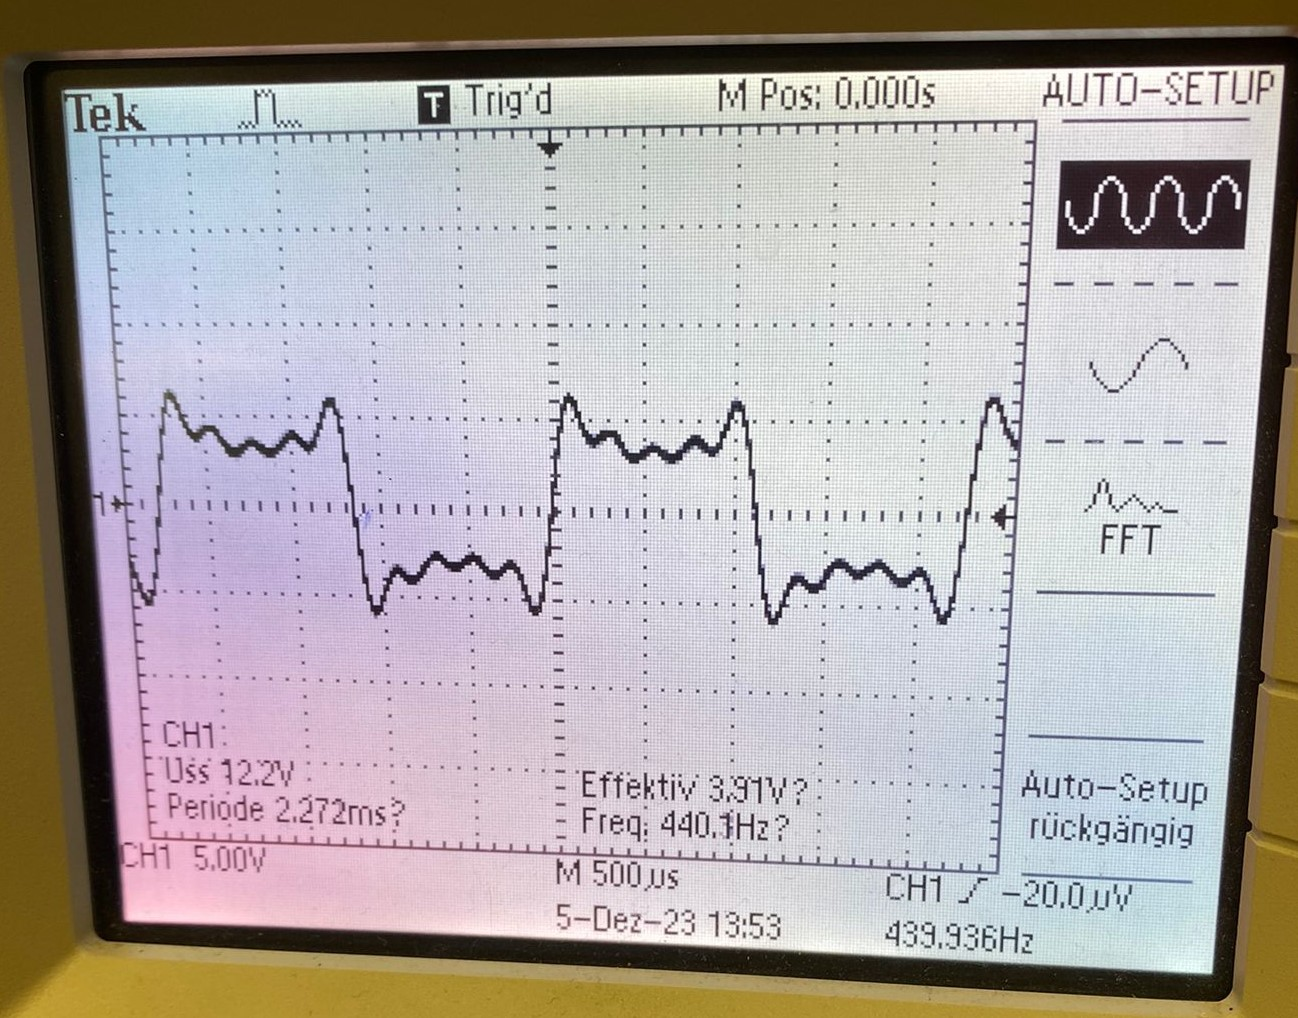
\includegraphics[height=7cm]{Bilder/recht.jpg}
  \caption{Ergebnis der Rechteckspannung mit Fourier-Synthese.}
  \label{fig:recht}
\end{figure}

Für die Dreieckspannung wurde die Funktion in Abbildung \ref{fig:drei} erreicht.

\begin{figure}[H]
  \centering
  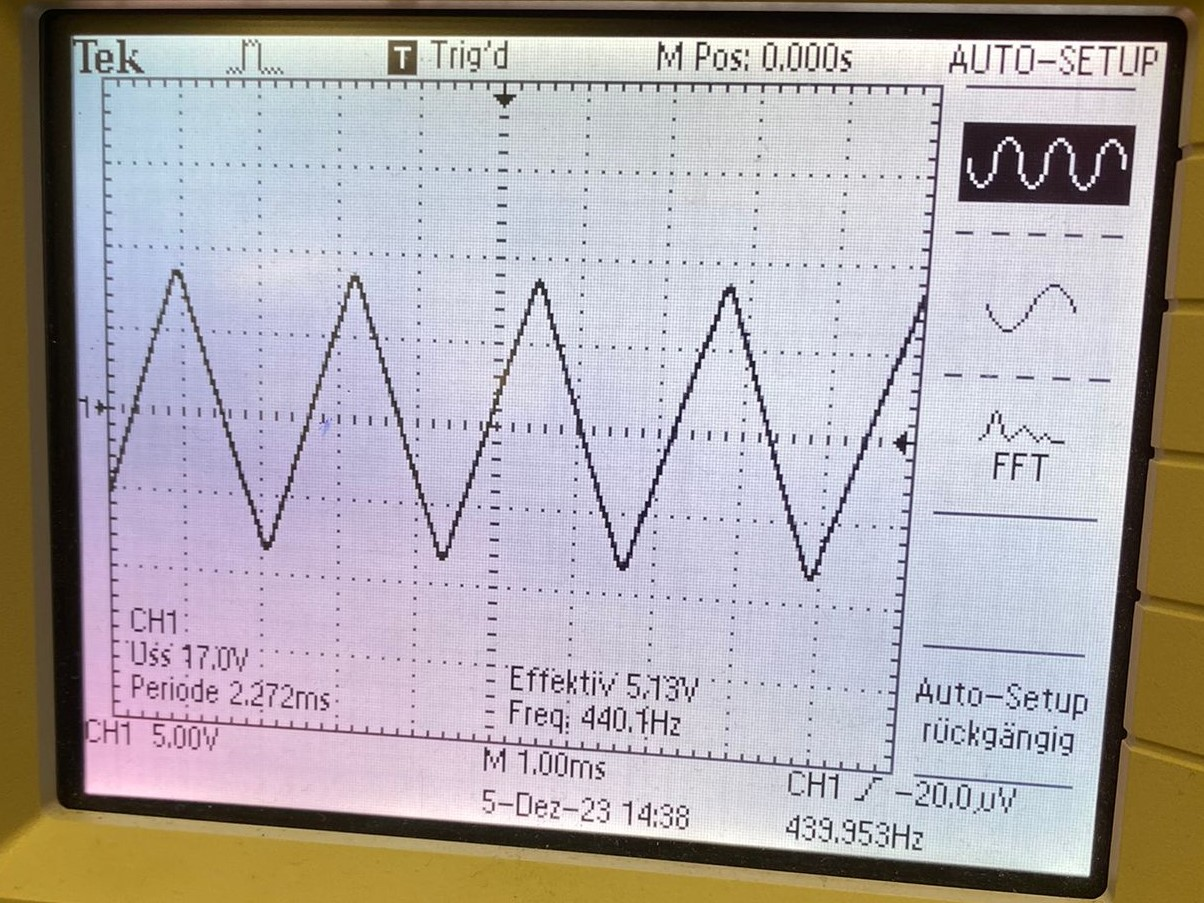
\includegraphics[height=7cm]{Bilder/drei.jpg}
  \caption{Ergebnis der Dreieckspannung mit Fourier-Synthese.}
  \label{fig:drei}
\end{figure}


Die Fourier-Synthese ergibt bei der Sägezahnspannung den Plot in Abbildung \ref{fig:säge}.
\begin{figure}[H]
  \centering
  \includegraphics[height=7cm]{Bilder/säge.jpg}
  \caption{Ergebnis der Sägezahnspannung mit Fourier-Synthese.}
  \label{fig:säge}
\end{figure}

\subsection{Fourier-Analyse}
Für die Fourier-Analyse wurden die Werte in Tabelle \ref{tab:tabelle4} gemessen. 
Zusätzlich wurden theoretische Werte mit den Formeln \ref{eqn:b_recht}, \ref{eqn:b_säge} und \ref{eqn:b_drei} berechnet.
Mit den theoretischen und experimentellen Werten wurde dann die Abweichung mit 
\begin{equation}
  |A|=\Bigl|\frac{b_{n,e}-b_{n,t}}{b_n,t}\Bigr|
  \label{eqn:abweichung}
\end{equation}
bestimmt.

\begin{table}[htbp]
  \centering
  \caption{Messwerte der Amplituden in Abhängigkeit zur Frequenz von der Rechteckspannung, der Sägezahnspannung und der Dreieckspannung.}
  \label{tab:tabelle4}
  \begin{minipage}[t]{0.5\linewidth}
  \begin{tblr}[t]{
    colspec={S[table-format=3.0] S[table-format=2.2] S[table-format=2.1] S[table-format=1.2] },
    row{1}={guard, mode=math},
    }
    \toprule
      f \mathbin{/} \unit{\kilo\hertz} &  b_{n,R,e} \mathbin{/} \unit{\volt}&  b_{n,R,t} \mathbin{/} \unit{\volt} & A_{e,t} \mathbin{/} \unit{\percent} \\
    \midrule
    
    10  & 89.13 &    89.1 & 0.03 \\
    30  & 29.51 &    29.7 & 0.63\\
    50  & 17.78 &    17.8 & 0.10\\
    70  & 12.88 &    12.7 & 1.44\\
    90  & 10.23 &     9.9 & 3.36\\
    110 &  8.13 &     8.1 & 0.35\\
    130 &  7.08 &     6.9 & 2.60\\
    150 &  6.17 &     5.9 & 4.51\\
    170 &  5.37 &     5.2 & 3.28\\
    190 &  4.90 &     4.7 & 4.21\\ 
    \bottomrule
  \end{tblr}
  
\end{minipage}
\hfill
\begin{minipage}[t]{0.5\linewidth}
  \begin{tblr}[t]{
    colspec={S[table-format=3.0] S[table-format=2.2] S[table-format=2.1] S[table-format=1.2] },
    row{1}={guard, mode=math},
    }
    \toprule
    f \mathbin{/} \unit{\kilo\hertz} &  b_{n,S,e} \mathbin{/} \unit{\volt}&  b_{n,S,t} \mathbin{/} \unit{\volt} & A_{e,t} \mathbin{/} \unit{\percent} \\
    \midrule
    10    & 44.67  &  44.7 & 0.07 \\
    20    & 22.39  &  22.3 & 0.39\\
    30    & 14.79  &  14.9 & 0.73 \\
    40    & 11.22  &  11.2 & 0.18 \\
    50    & 8.91   &   8.9 & 0.14 \\
    60    & 7.41   &   7.4 & 0.18 \\
    70    & 6.46   &   6.4 & 0.88 \\
    80    &  5.62  &   5.6 & 0.42 \\
    90    &  5.13  &   5.0 & 2.57 \\
    100   &  4.47  &   4.5 & 0.74 \\
    \bottomrule
  \end{tblr}

\end{minipage}
\hfill
  \begin{minipage}[t]{0.5\linewidth}
  \begin{tblr}[t]{
    colspec={S[table-format=3.0] S[table-format=2.2] S[table-format=2.1] S[table-format=1.2] },
    row{1}={guard, mode=math},
    }
    \toprule
    f \mathbin{/} \unit{\kilo\hertz} &  b_{n,D,e} \mathbin{/} \unit{\volt}&  b_{n,D,t} \mathbin{/} \unit{\volt} & A_{e,t} \mathbin{/} \unit{\percent} \\
    \midrule
    
    10 & 56.23  &   56.20 & 0.06 \\
    30 &  6.17  &    6.20 & 0.55\\
    50 &  2.35  &    2.20 & 6.68\\
    70 &  1.12  &    1.15 & 2.32\\
    \bottomrule
  \end{tblr}
  
\end{minipage}
\hfill
\end{table}

Die Werte für die Amplituden werden mit der Formel
\begin{equation*}
  \unit{\volt}=10^{\frac{\unit{\decibel}}{20}}
\end{equation*}
von Dezibel in Volt umgerechnet.
Diese werden dann in Abbildung \ref{fig:plot1} geplottet.
Dazu werden noch die Theoriewerte geplottet, die mit den Formeln \ref{eqn:b_recht}, \ref{eqn:b_drei} und \ref{eqn:b_säge} berechnet werden.

\begin{figure}
  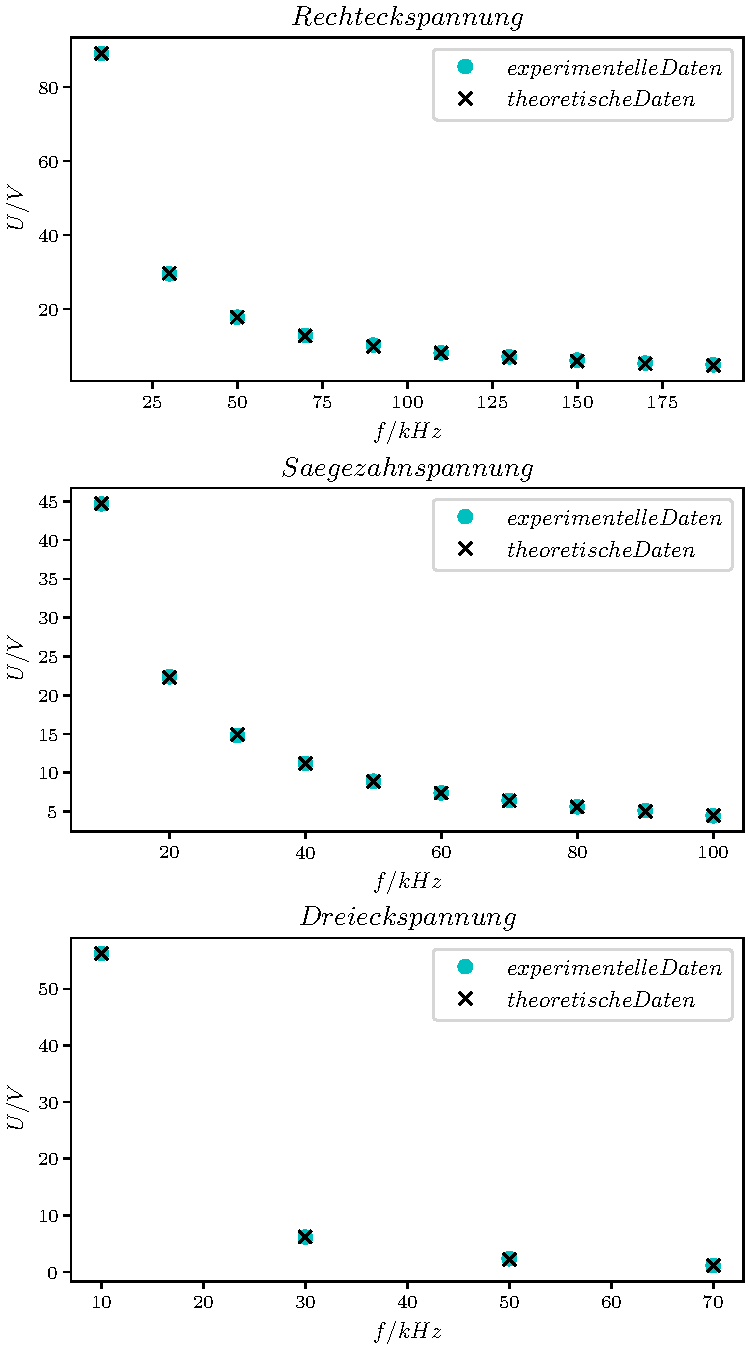
\includegraphics[width=\textwidth, height=20cm]{plot1.pdf}
  \label{fig:plot1}
\caption{Hier sind die Graphen von Experimental- und Theoriewert der Amplituden in Volt gegen die Frequenz im Kilohertz aufgetragen.}
\end{figure}



